\documentclass[11pt, a4paper]{article}
\usepackage{ModernTeX}




\begin{document}
\sloppy

\title{Optimering 1}

\author{Trym Sæther}

\maketitle

\tableofcontents

\newpage

\section{Introduksjon til optimering}

\subsection{Optimeringsproblemet}
La $f: \Omega \to \R$ være en (objekt)funksjon som vi ønsker å maksimere eller minimere, der $\Omega \subset \R^d$ er en ikke-tom mengde (feasible set).

\begin{definition}{Optimeringsproblemet \((P)\)}{}
    \[
        \min_{x \in \Omega} f(x) \quad \text{eller} \quad \max_{x \in \Omega} f(x).
    \]\label{def:optimization_problem}
\end{definition}


\section{Fri optimalisering}

Fri optimalisering refererer til problemer uten eksplisitte restriksjoner på variablene. Målet er å minimere en glatt objektiv funksjon \( f : \mathbb{R}^n \to \mathbb{R} \) over hele rommet \( \mathbb{R}^n \). Problemformuleringen er:

\[
    \min_{x \in \mathbb{R}^n} f(x),
\]
der løsningen \( x^* \) tilfredsstiller:
\[
    f(x^*) \leq f(x), \quad \forall x \in \mathbb{R}^n.
\]

\subsection*{Egenskaper}

\begin{itemize}
    \item \textbf{Ingen restriksjoner}: Den tillatte mengden (feasible set) er hele \( \mathbb{R}^n \), uten likhets- eller ulikhetsbetingelser.
    \item \textbf{Enklere oppsett}: Det er ikke behov for å håndtere restriksjoner som sikrer at løsningen er gyldig.
    \item \textbf{Fokuserer kun på målfunksjonen}: Algoritmer søker etter punkter \( x \) som reduserer \( f(x) \) direkte, uten å ta hensyn til andre forhold.
\end{itemize}

\subsection*{Konvergens}
For å sikre konvergens til en stasjonær løsning \( x^* \), må følgende betingelser oppfylles:
\begin{enumerate}
    \item \( f(x) \) er kontinuerlig deriverbar (\( C^1 \)), og dens gradient \( \nabla f(x) \) eksisterer og er Lipschitz-kontinuerlig.
    \item Nivåsettene \( \{x \in \mathbb{R}^n : f(x) \leq c\} \) er kompakte.
\end{enumerate}

Under disse betingelsene sikres:
\[
    \lim_{k \to \infty} \|\nabla f(x_k)\| = 0,
\]

der \( x_k \) er iteratene generert av en optimaliseringsalgoritme. Akkumuleringspunkter \( x^* \) tilfredsstiller førsteordens nødvendige betingelser:
\[
    \nabla f(x^*) = 0.
\]

\section{Begreper og definisjoner}

\subsection{Nivåsett}

$f: \Omega \to \overline{\R}$ er en funksjon. Vi definerer nivåsettet til $f$ i punktet $y \in \R$ som:

\begin{definition}{Nivåsett}{level_set}
    \[
        \mathcal{L}_f(y) = \{x \in \Omega | f(x) = y\}.
    \]
\end{definition}

\begin{definition}{Nedre semi-kontinuerlig funksjoner}{lsc}

    $f: \Omega (\subset \R^d) \to \overline{\R}$ være en funksjon. Vi sier at $f$ er nedre semi-kontinuerlig (lsc) i punktet $x_0$ hvis for alle $\varepsilon > 0$ finnes det en $\delta > 0$ slik at

    \[
        f(x) > f(x_0) - \varepsilon \quad \text{for alle} \quad x \in B(x_0, \delta).
    \]

    \begin{enumerate}
        \item $f$ er (lsc) i $x_0$ hvis det for alle $\alpha \in \R$ er mengden $\mathcal{L}_f(\alpha) = \{x | f(x) < \alpha \} \text{ er åpen i } \R^d$
        \item $f$ er (lsc) i $x_0 \in X$ hvis og bare hvis: $\liminf_{x \to x_0} f(x) \geq f(x_0)$.
    \end{enumerate}

\end{definition}

\begin{example}{(lsc)}{}
    \begin{figure}[H]
        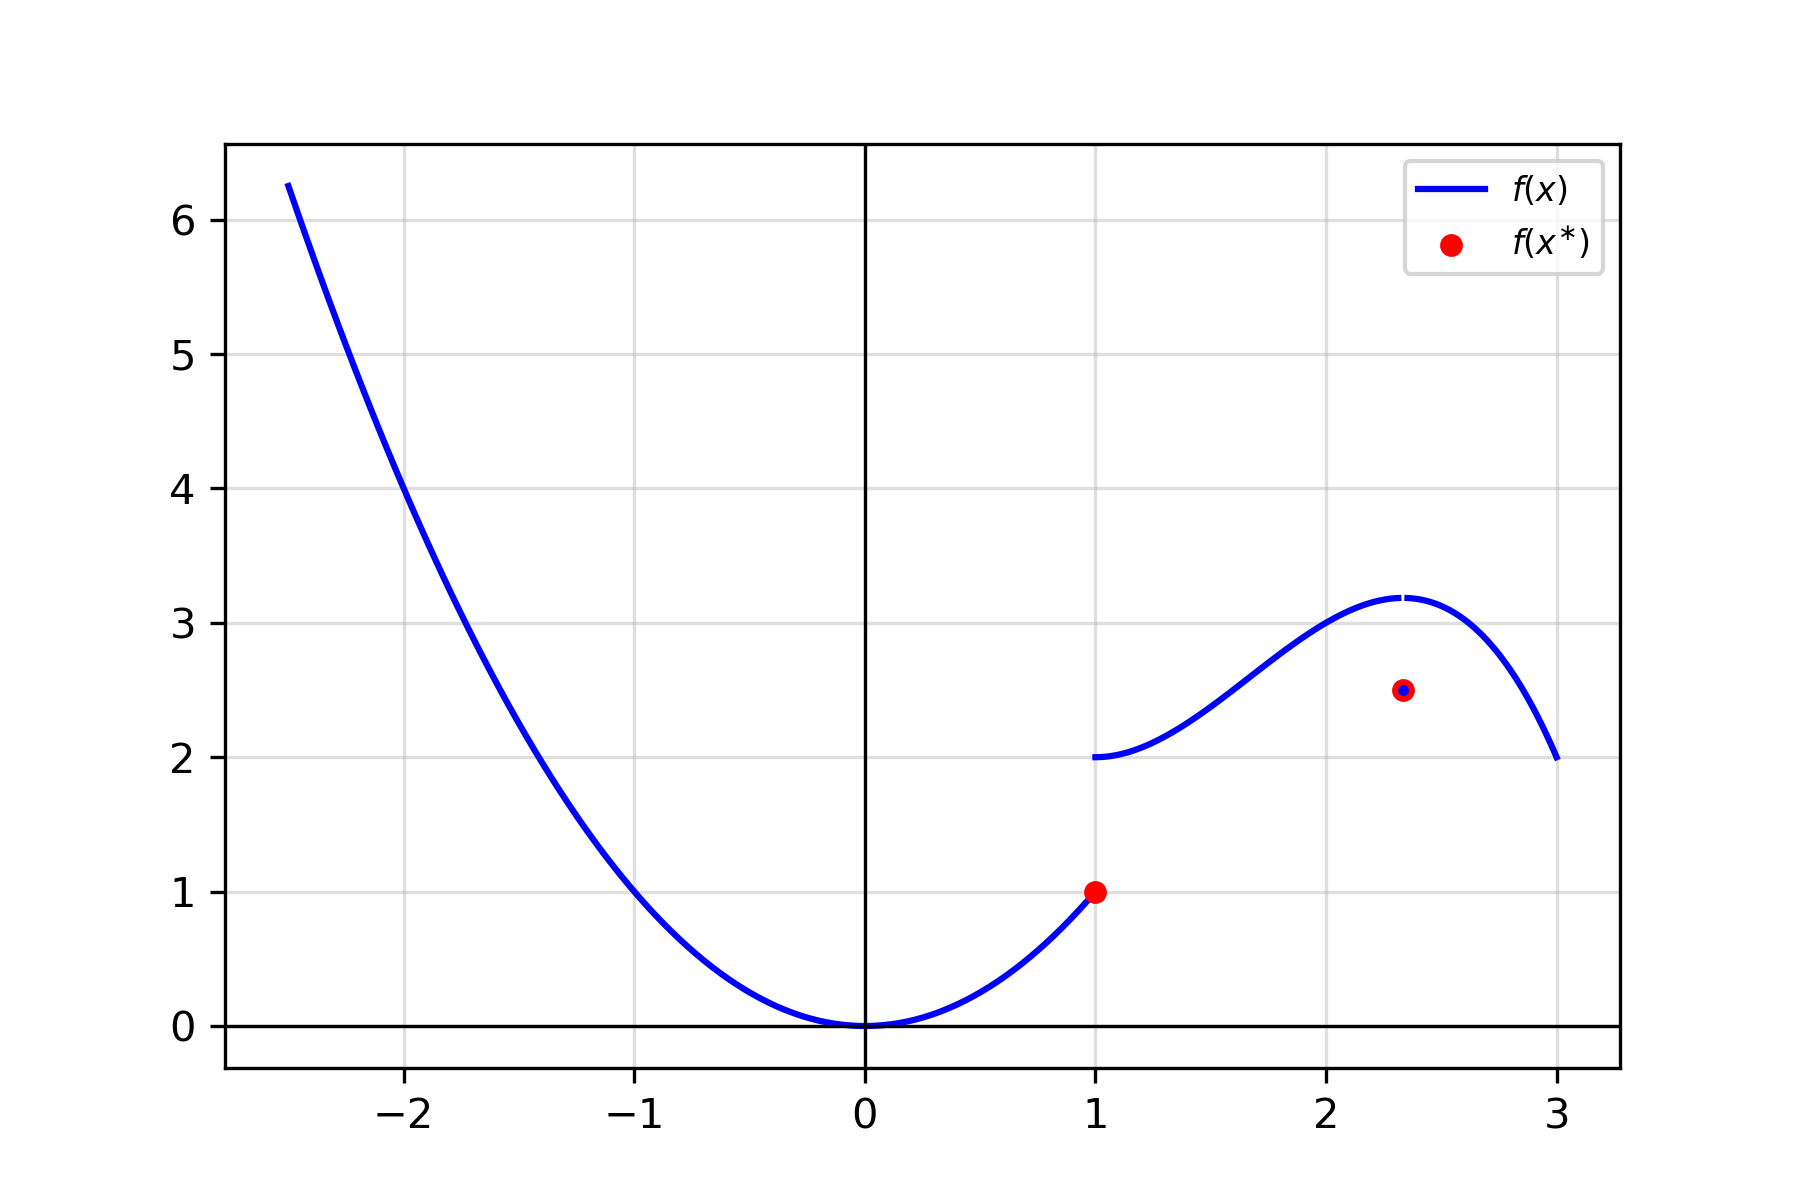
\includegraphics[scale=0.7]{figures/example_lsc.png}
        \caption{Eksempel på en nedre semi-kontinuerlig funksjon.}
        \label{fig:lsc}
    \end{figure}
\end{example}

\begin{definition}{Koersivitet}{}
    $f: \Omega \to \overline{\R}$ er en koersiv funksjon hvis for alle $y \in \R$ er nivåmengden $f^{-1}(y)$ kompakt i $\Omega$.
\end{definition} \label{def:coercive}

\subsection{Konveksitet}

\begin{definition}{Konveks funksjon}{convex_function}
    En funksjon $f: \R^n \to \R$ er konveks hvis for alle $x, y \in \R^n$ og $\lambda \in [0, 1]$ har vi:

    \begin{align*}
        f(\lambda x + (1 - \lambda)y) & \leq \lambda f(x) + (1 - \lambda)f(y) \tag{Konveks} \\
    \end{align*}

    \begin{filingbox}[colback=red!20!white][Strengt konveks]{Strengt konveks funksjon}
        En funksjon $f: \R^n \to \R$ er strengt konveks hvis for alle $x, y \in \R^n$ og $\lambda \in (0, 1)$ har vi:
        \[
            f(\lambda x + (1 - \lambda)y) < \lambda f(x) + (1 - \lambda)f(y)
        \]\label{def:strictly_convex}
    \end{filingbox}
    \begin{filingbox}(ul)[red!20!white]{Kvasi-konveks}
        En funksjon $f: \R^d \to \R$ er kvasi-konveks hvis for alle $x, y \in \R^n$ og $\lambda \in (0, 1)$ har vi:

        \[
            f(\lambda x + (1 - \lambda)y) \leq \max\{f(x), f(y)\}
        \]

        En alternativ definisjon er at en funksjon er kvasi-konveks hvis alle nivåsettene er konvekse.

        \[
            \mathcal{L}_f(y) = \{x \in \R^n | f(x) \leq y\} \quad \text{er konveks for alle} \quad y \in \R
        \]

        \[
            \boxed{\underbrace{\forall \alpha \in \mathbb{R}, \mathcal{L}_f(\alpha) \text{ er konveks}}_{f \text{ er kvasi-konveks }}\Longleftrightarrow \forall x, y \in \mathbb{R}^d,\lambda \text{ s.a. } f(\lambda x + (1-\lambda)y) \leq \max \{ f(x), f(y) \}}
        \]
    \end{filingbox}\label{def:quasi_convex}

\end{definition}

En mengde $C \subset \R^n$ er (strengt) konveks når:

\begin{definition}{Konveks sett}{convex_set}

    \begin{align*}
        \lambda x + (1 - \lambda)y & \in C \quad \forall \; x, y \in C, \lambda \in [0, 1] \tag{Konveks}                   \\
        \lambda x + (1 - \lambda)y & \in C \quad \forall \; x, y \in C, \lambda \in (0, 1), x \neq y \tag{Strengt konveks}
    \end{align*}

\end{definition}


\subsection{Globale og lokale løsninger}

La $f: \Omega \to \R$ være en funksjon. Vi sier at $x^* \in \Omega$ er en global løsning av minimeringsproblemet \((P)\) hvis

\begin{definition}{Global løsning}{}
    \begin{align*}
        f(x^*) & \leq f(x) \quad \text{for alle} \quad x \in \Omega, \tag{Global løsning}                 \\
        f(x^*) & < f(x) \quad \text{for alle} \quad x \in \Omega, x \neq x^*. \tag{Streng global løsning}
    \end{align*}
\end{definition}

La $f: \Omega \to \R$ være en funksjon. Vi sier at $x^* \in \Omega$ er en lokal løsning av optimeringsproblemet hvis

\begin{definition}{Lokal løsning}{}
    \begin{align*}
        f(x^*) & \leq f(x) \quad \text{for alle} \quad x \in B(x^*, \varepsilon) \cap \Omega, \tag{Lokal løsning}                     \\
        f(x^*) & < f(x) \quad \text{for alle} \quad x \in B(x^*, \varepsilon) \cap \Omega, x \neq x^*. \tag{Streng lokal løsning}     \\
        f(x^*) & \leq f(x) \quad \text{for alle} \quad x \in B(x^*, \varepsilon) \cap \Omega, x \neq x^*. \tag{Isolert lokal løsning}
    \end{align*}
\end{definition}

\begin{remark}{Maksimeringsproblemet}{}
    for maksimeringsproblemer snur vi bare ulikhetene.
    \[
        \leq \; \leftrightarrow \; \geq
    \]
\end{remark}

\subsection*{Eksistens av globale løsninger}

Hvis $f: \Omega \subset \R^d \to \overline{\R}$ er nedre semi-kontinuerlig og koersiv på $\Omega$, så har $f$ en global løsning (minimum) i $\Omega$.

\begin{enumerate}
    \item $f$ er nedre semi-kontinuerlig (lsc) på $\Omega$ hvis for alle $y \in \R$ er nivåmengden $f^{-1}(y)$ lukket i $\Omega$.
    \item $f$ er koersiv på $\Omega$ hvis for alle $y \in \R$ er nivåmengden $f^{-1}(y)$ kompakt i $\Omega$.
    \item $f$ er konveks på $\Omega$ hvis for alle $x, y \in \Omega$ og $\lambda \in [0, 1]$ har vi:
    \item
          \[
              f(\lambda x + (1 - \lambda)y) \leq \lambda f(x) + (1 - \lambda)f(y).
          \]
\end{enumerate}

\newpage
\section{Funksjoner}
\begin{table}[ht]
    \centering
    \caption{Function Properties and Optimization Methods (Corrected)}
    \label{tab:function_properties}
    \footnotesize
    \begin{tabularx}{\textwidth}{@{} >{\RaggedRight}Z Y Y Y Y Y Y Y @{}}
        \toprule
        \textbf{Function (Domain)}                                                        & \textbf{Cvx} & \textbf{Coe} & \textbf{lsc} & \textbf{QCvx} & \textbf{Loc} & \textbf{Glo} & \textbf{Alg}         \\
        \midrule

        \multicolumn{8}{@{}l}{\textbf{Scalar Functions (\(\mathbb{R}\))}}                                                                                                                                   \\
        \midrule
        \( f(x) = x^2 \)                                                                  & \yes         & \yes         & \yes         & \yes          & \yes         & \yes         & Gradient Descent     \\
        \( f(x) = |x| \)                                                                  & \yes         & \yes         & \yes         & \yes          & \yes         & \yes         & Proximal/Subgradient \\
        \( f(x) = x^3 \)                                                                  & \no          & \no          & \yes         & \no           & \no          & \no          & Heuristics           \\
        \( f(x) = x^4 - Cx^2 \)                                                           & \no          & \yes         & \yes         & \no           & \yes         & \yes         & Newton               \\
        \( f(x) = \begin{cases} 0 & x \leq 0 \\ 1 & x > 0 \end{cases} \)                  & \no          & \no          & \yes         & \yes          & \yes         & \yes         & Subgradient          \\

        \( f(x) = \sqrt{x}\ (x \geq 0) \)                                                 & \no          & \no          & \yes         & \yes          & \yes         & \yes         & Gradient Descent     \\
        \( f(x) = \log(1 + e^x) \)                                                        & \yes         & \yes         & \yes         & \yes          & \yes         & \yes         & Gradient Descent     \\
        \( f(x) = Ce^x \)                                                                 & \yes         & \no          & \yes         & \yes          & \no          & \no          & Heuristics           \\
        \( f(x) = e^x - x \)                                                              & \yes         & \yes         & \yes         & \yes          & \yes         & \yes         & Newton               \\
        \( f(x) = \sin(x) \)                                                              & \no          & \no          & \yes         & \no           & \yes         & \yes         & Heuristics           \\

        \midrule

        \multicolumn{8}{@{}l}{\textbf{Vector Functions (\(\mathbb{R}^d\))}}                                                                                                                                 \\
        \midrule
        \( f(\mathbf{x}) = \|\mathbf{x}\| \)                                              & \yes         & \yes         & \yes         & \yes          & \yes         & \yes         & Proximal             \\
        \( f(\mathbf{x}) = \|\mathbf{x}\| + \sin(x_1) \)                                  & \no          & \yes         & \yes         & \no           & \yes         & \yes         & Stochastic GD        \\
        \( f(\mathbf{x}) = \mathbf{x}^\top \mathbf{A} \mathbf{x}\ (\mathbf{A} \succ 0) \) & \yes         & \yes         & \yes         & \yes          & \yes         & \yes         & Newton               \\
        \midrule

        \multicolumn{8}{@{}l}{\textbf{Counterexamples}}                                                                                                                                                     \\
        \midrule
        \( f(x) = \sqrt{|x|} \)                                                           & \no          & \no          & \yes         & \yes          & \no          & \no          & Heuristics           \\
        \( f(x,y) = x^4y^2 + x^4 - 2x^3y \)                                               & \no          & \yes         & \yes         & \no           & \yes         & \yes         & Evolutionary         \\
        \bottomrule
    \end{tabularx}
    \vspace{0.5em}
    \footnotesize
    \textbf{Key Corrections:}
    \begin{itemize}
        \item \( f(x) = |x| \): Marked as convex/coercive; algorithm changed to Proximal/Subgradient.
        \item \( f(x) = x^3 \): Corrected coerciveness (No) and minima (No).
        \item \( f(x) = \sqrt{x} \): Added domain restriction \( x \geq 0 \); has global minimum at 0.
        \item \( f(x) = \sin(x) \): Quasi-convexity corrected to No; has infinite global minima.
        \item Quadratic forms: Explicitly stated \( \mathbf{A} \succ 0 \) for convexity.
    \end{itemize}
\end{table}

\newpage
\begin{table}[ht]
    \centering

    \label{tab:glossary}
    \footnotesize
    \begin{tabularx}{\textwidth}{@{}>{\color{black!70}}l>{\raggedright\arraybackslash}X@{}}
        \toprule
        \rowcolor{headerblue}
        \textbf{Term}     & \textbf{Definition/Formula}                                                                                                                               \\
        \midrule

        Convex            & \( f(\lambda x + (1-\lambda)y) \leq \lambda f(x) + (1-\lambda)f(y), \ \forall x,y \in \R^d, \lambda \in [0,1] \)                                          \\

        Coercive          & \( \lim_{\|x\| \to \infty} f(x) = \infty \) (ensures existence of minima)                                                                                 \\

        lsc               & \( \liminf_{x \to x_0} f(x) \geq f(x_0) \) (sublevel sets closed)                                                                                         \\

        Quasi-Convex      & \( \mathcal{L}_{f}(\alpha) = \{x \mid f(x) \leq \alpha\} \text{ convex } \forall \alpha \in \R \iff f(\lambda x + (1-\lambda)y) \leq \max\{f(x),f(y)\} \) \\

        Local Minimum     & \( \exists \epsilon > 0: f(x^*) \leq f(x), \, \forall x \in B_\epsilon(x^*) \)                                                                            \\

        Global Minimum    & \( f(x^*) \leq f(x), \, \forall x \in \R^d \)                                                                                                             \\

        Proximal Operator & \( \text{prox}_{\gamma f}(v) = \arg\min_x \left( f(x) + \frac{1}{2\gamma}\|x - v\|^2 \right) \)                                                           \\

        Subgradient       & \( g \in \partial f(x) \text{ if } f(y) \geq f(x) + g^\top(y-x), \, \forall y \in \R^d \)                                                                 \\

        Stochastic GD     & \( x_{k+1} = x_k - \eta_k \nabla f_{i_k}(x_k) \) (randomized gradients)                                                                                   \\

        Newton's Method   & \( x_{k+1} = x_k - [\nabla^2 f(x_k)]^{-1} \nabla f(x_k) \)                                                                                                \\
        \bottomrule
    \end{tabularx}
    \caption{Quick Reference: Key Definitions and Formulas}
\end{table}


\section{Lectures}

\subsubsection{Lecture 1 (6. Januar 2025)}

\section*{Eksistens av globale løsninger}

\begin{definition}{Nivåmengde}{level-set}
  For en funksjon $f: \mathbb{R}^d \to \mathbb{R}$ definerer vi nivåmengden som
  \[
    L_f(\alpha) = \{x \in \R^d : f(x) \leq \alpha\}
  \]
\end{definition}

\begin{theorem}{Karakterisering av koersivitet og semi-kontinuitet}{characterization}
  La $f: \mathbb{R}^d \to \mathbb{R}$ være en funksjon. Da har vi:
  \begin{itemize}
    \item $f$ er koersiv $\iff L_f(\alpha)$ er avgrenset for alle $\alpha < \infty$
    \item $f$ er nedre semi-kontinuerlig (lsc) $\iff L_f(\alpha)$ er lukket for alle $\alpha$
  \end{itemize}
\end{theorem}

\begin{theorem}{Eksistens av globale løsninger}{existence}
  Hvis $f: \mathbb{R}^d \to \mathbb{R}$ er koersiv og nedre semi-kontinuerlig, så har problemet
  \[
    \min_{x \in \mathbb{R}^d} f(x)
  \]
  en global løsning.
\end{theorem}

\section*{Nødvenige og tilstrekkelige betingelser for lokale løsninger}

\begin{theorem}{Nødvendige betingelser for lokale løsninger}{necessary-conditions}
  La $x^* \in \mathbb{R}^d$ være en lokal løsning av $\min_{x \in \mathbb{R}^d} f(x)$. Da gjelder:
  \begin{itemize}
    \item $\nabla f(x^*) = 0$ (Førsteordens nødvendig betingelse).
    \item $H_f(x^*)$ er positiv semi-definit (Andreordens nødvendig betingelse).
  \end{itemize}
  da er $x^*$ en lokal løsning av $\min_{x \in \mathbb{R}^d} f(x)$.
\end{theorem}\label{thm:necessary-conditions}

\begin{theorem}{Tilstrekkelige betingelser for lokale løsninger}{sufficient-conditions}
  Hvis $x^* \in \mathbb{R}^d$ oppfyller:
  \begin{itemize}
    \item $\nabla f(x^*) = 0$ (Førsteordens betingelse)
    \item $H_f(x^*)$ er positiv definit (Andreordens tilstrekkelig betingelse)
  \end{itemize}
  da er $x^*$ en streng og isolert lokal løsning av $\min_{x \in \mathbb{R}^d} f(x)$.
\end{theorem}\label{thm:sufficient-conditions}

\begin{example}{Eksistens og optimalitet}{}
  \begin{itemize}
    \item For \( f(x) = x^2 + 2x \), som er kontinuerlig og koersiv, finnes et globalt minimum i \( x^* = -1 \) der \( f(-1) = -1 \).
    \item For \( f(x) = x^2 \), har vi \( \nabla f(x) = 2x \). I \( x^* = 0 \) er \( \nabla f(0) = 0 \) og \( \nabla^2 f(x) = 2 > 0 \), som oppfyller SOSC.
  \end{itemize}
\end{example}

\subsection{Lecture 2 (10. January 2025)}

\section*{Gradientmetoder og konveksitet}

\begin{theorem}{Gradientestimat nær lokale minima}{gradient-estimate}
  La $f: \mathbb{R}^n \to \mathbb{R}$ være deriverbar og $x^*$ være et lokalt minimum. Da gjelder:
  \[
    \|\nabla f(x)\| \to 0 \quad \text{når } x \to x^*.
  \]
\end{theorem}

\begin{remark}{Geometrisk tolkning}
  Dette indikerer at funksjonen blir "flatere" når $x$ nærmer seg minimumpunktet, noe som er fundamentalt for konvergensen til iterative optimaliseringsmetoder.
\end{remark}

\begin{definition}{Konveks funksjon}{convex-function}
  En funksjon $f: \mathbb{R}^n \to \mathbb{R}$ er konveks hvis, for alle $x, y \in \mathbb{R}^n$ og $\lambda \in (0,1)$:
  \begin{align*}
    f(\lambda x + (1 - \lambda)y) \leq \lambda f(x) + (1 - \lambda)f(y) \tag{Konveks} \\
    f(\lambda x + (1 - \lambda)y) < \lambda f(x) + (1 - \lambda)f(y) \tag{Strengt konveks}
  \end{align*}

\end{definition}

\begin{theorem}{Karakterisering av deriverbare konvekse funksjoner}{convex-characterization}
  For en deriverbar funksjon $f: \mathbb{R}^n \to \mathbb{R}$ er følgende ekvivalente:
  \begin{itemize}
    \item $f$ er konveks
    \item For alle $x, y \in \mathbb{R}^n$ gjelder:
          \[
            f(y) \geq f(x) + \nabla f(x)^\top (y - x)
          \]
  \end{itemize}
\end{theorem}

\begin{theorem}{Karakterisering av konvekse funksjoner med Hessian}{convex-hessian}
  For en dobbelt deriverbar funksjon $f: \mathbb{R}^n \to \mathbb{R}$ er følgende ekvivalente:
  \[
    f \text{ er konveks} \iff H_f(x) \succeq 0 \quad \forall x \in \mathbb{R}^n
  \]

  $H_f(x) \succeq 0$ betyr at Hessian-matrisen er positiv semi-definit for alle $x$.

\end{theorem}

\begin{remark}{Positiv semi-definit matrise}
  En matrise $A \in \mathbb{R}^{n \times n}$ er positiv semi-definit hvis og bare hvis en av følgende ekvivalente påstander holder:
  \begin{align*}
    A \succeq 0 & \iff x^\top A x \geq 0 \quad \forall x \in \mathbb{R}^n \tag{Kvadratisk form}                     \\
                & \iff \lambda_i \geq 0 \text{ for alle egenverdier } \lambda_i \text{ av } A \tag{Egenverdier}     \\
                & \iff \text{Alle hovedminordeterminanter er ikke-negative} \tag{Minordeterminanter}                \\
                & \iff A = LL^\top \text{ for en nedre triangulær matrise } L \tag{Cholesky}                        \\
                & \iff A = B^\top B \text{ for en matrise } B \in \mathbb{R}^{m \times n} \tag{Gram}                \\
                & \iff A - 0 \cdot I \succeq 0 \tag{Semidefinit ordning}                                            \\
                & \iff A \text{ ligger i den positive semidefinite konen i } \mathbb{R}^{n \times n} \tag{PSD kone} \\
                & \iff e^{tA} \text{ er positiv semidefinit for alle } t > 0 \tag{Matrise eksponential}
  \end{align*}

  \begin{itemize}
    \item Kvadratisk form: $x^\top A x \geq 0$ for alle $x \in \mathbb{R}^n$ karakteriserer positiv semi-definite matriser.
    \item Egenverdier: Alle egenverdier $\lambda_i$ av $A$ er ikke-negative.
    \item Hovedminordeterminant: Determinanten til alle hoved-undermatriser er ikke-negative.
          \[
            \begin{bmatrix}
              a_{11} & a_{12} \\
              a_{21} & a_{22}
            \end{bmatrix} \succeq 0 \iff a_{11} \geq 0, \quad a_{11}a_{22} - a_{12}a_{21} \geq 0
          \]

    \item Cholesky-faktorisering: $A = LL^\top$ der $L$ er en nedre triangulær matrise.
    \item Gram-matrise: $A = B^\top B$ der $B \in \mathbb{R}^{m \times n}$.
    \item Semidefinit ordning: $A - 0 \cdot I \succeq 0$ betyr at $A$ er positiv semi-definit.
    \item PSD-kone: Den positive semidefinite konen er mengden av alle positiv semi-definite matriser.
    \item Matrise eksponential: $e^{tA}$ er positiv semi-definit for alle $t > 0$.
  \end{itemize}
\end{remark}


\begin{theorem}{Globale egenskaper for konvekse funksjoner}{global-properties}
  La $f: \mathbb{R}^n \to \mathbb{R}$ være konveks. Da gjelder:
  \begin{itemize}
    \item Ethvert lokalt minimum er også et globalt minimum.
    \item Hvis $\nabla f(x^*) = 0$, da er $x^*$ et globalt minimum.
  \end{itemize}
\end{theorem}

\begin{example}{Konvekse funksjoner}{convex-examples}
  Noen klassiske eksempler på konvekse funksjoner:
  \begin{itemize}
    \item Lineære funksjoner: $f(x) = a^\top x + b$
    \item Kvadratiske funksjoner med positiv definit matrise: $f(x) = x^\top Ax + b^\top x + c$, der $A \succ 0$
    \item Eksponentialfunksjonen: $f(x) = e^{ax}$ for enhver $a \in \mathbb{R}$
  \end{itemize}
\end{example}


\subsection{Lecture 3 (13. January 2025)}
\section*{Optimization Algorithms}

\begin{definition}{Nelder-Mead Algorithm}{nelder-mead}
  The Nelder-Mead algorithm is a heuristic search method used for minimizing an objective function without the need for derivatives. It operates on a simplex of \( n+1 \) points in \( \mathbb{R}^n \) and iteratively reflects, expands, contracts, or shrinks the simplex to converge to a local minimum.

\end{definition}

\begin{algorithm}[H]
  \caption{Nelder-Mead Algorithm}
  \label{alg:nelder-mead}
  Initialize simplex with $n+1$ points\;
  \Repeat{convergence criteria are met}{
    Order the simplex points by their objective function values\;
    Compute the centroid of the best $n$ points\;
    Reflect the worst point through the centroid\;
    \uIf{reflected point is better than the second worst but not better than the best}{
      Accept the reflection\;
    }
    \uElseIf{reflected point is the best point}{
      Try expanding\;
    }
    \uElseIf{reflected point is worse than the second worst}{
      Perform contraction\;
    }
    \Else{
      Shrink the simplex towards the best point\;
    }
  }
\end{algorithm}

\subsubsection*{line search methods}
Line search methods aim to find an appropriate step size \( \alpha \) that sufficiently decreases the objective function along a given search direction \( d \). The goal is to ensure convergence and improve the efficiency of optimization algorithms.

\subsubsection*{Gradient Descent and Newton Directions}

\begin{definition}{Gradient Descent}{gradient-descent}
  Gradient descent is an iterative optimization algorithm that updates the current point \( x_k \) by moving in the opposite direction of the gradient:
  \[
    x_{k+1} = x_k - \alpha_k \nabla f(x_k)
  \]
  where \( \alpha_k \) is the step size.
\end{definition}

\begin{definition}{Newton Direction}{newton-direction}
  Newton's method uses second-order information by incorporating the Hessian matrix:
  \[
    x_{k+1} = x_k - [\nabla^2 f(x_k)]^{-1} \nabla f(x_k)
  \]
  This direction can provide faster convergence near the optimum.
\end{definition}

\subsubsection*{Armijo Condition for Step-Length Selection}

\begin{definition}{Armijo Condition}{armijo}
  The Armijo condition ensures that the step size \( \alpha \) provides a sufficient decrease in the objective function:
  \[
    f(x_k + \alpha d_k) \leq f(x_k) + c \alpha \nabla f(x_k)^\top d_k
  \]
  where \( 0 < c < 1 \) is a constant.
\end{definition}

\subsubsection*{Backtracking Line Search}

\begin{definition}{Backtracking Line Search}{backtracking}
  Backtracking line search starts with an initial step size and iteratively reduces it by a factor until the Armijo condition is satisfied.

\end{definition}

\begin{algorithm}[H]
  \caption{Backtracking Line Search}
  \label{alg:backtracking}
  \SetKwFunction{BacktrackingLineSearch}{BacktrackingLineSearch}
  \BacktrackingLineSearch{$x_k$, $d_k$, $f$, $\nabla f$, $\alpha$, $\rho$, $c$}\;
  \While{$f(x_k + \alpha d_k) > f(x_k) + c \alpha \nabla f(x_k)^\top d_k$}{
    $\alpha \gets \rho \alpha$\;
  }
  \KwRet{$\alpha$}\;
\end{algorithm}
\newpage

\subsection{Lecture 4 (17. Januar 2025)}

\subsubsection*{Numerical methods for free optimization}

\textbf{Goal:}

We want to solve \( \min_{x \in \R^d} f(x) \) numerically. Want to find an approximate solution to the problem with:

\begin{itemize}
    \item Good accuracy
    \item sufficiently fast
\end{itemize}

\textbf{Assumption:} Given $ x \in \R^d $, we have a black-box that computes $f(x), \nabla f(x), \nabla^2 f(x) , \ldots $.

\textbf{Can expect:}
\begin{itemize}
    \item calculation of \(f(x)\) is much more expensive than additions/multiplications/divisions of \(x\).
    \item calculation of \(\nabla f(x)\) is more expensive than \(f(x)\).
\end{itemize}

It should try to minimize the number of function and gradient evaluations.

\subsection*{Nelder-Mead Algorithm}
\textbf{Properties:}
\begin{itemize}
    \item Derivative-free method
    \item Only require $f(x)$, but not $\nabla f(x)$.
          \begin{itemize}
              \item $\nabla f(x)$ might be to expensive to compute.
              \item $\nabla f(x)$ might be unavailable.
              \item $f(x)$ might not be differentiable.
          \end{itemize}
    \item Works well for low-dimensional problems, but not for high-dimensional problems.
\end{itemize}

\textbf{Idea of Nelder-Mead:}
Choose $d+1$ affinely independent points in $\R^d$.
\begin{align*}
    x_1, x_2, \ldots, x_{d+1} \in \R^d \\
    f(x_1) \leq f(x_2) \leq \ldots \leq f(x_{d+1})
\end{align*}
Then replace the worst point $x_{d+1}$ with a better point:

define $\bar{x} := \frac{1}{d} \sum_{k=0}^{d-1} x_k$ and choose a new point on the line $\bar{x} - t(x_{d} - \bar{x})$ with $t < 1$.

Take particularly: $t= -1$, $t = -2$, $t = 0.5$ or $t = 0.5$.

\begin{itemize}
    \item \textit{If:} one of these points $f(x_k)$ is better than $f(x_{d})$, replace $x_{d}$ by this point.
    \item \textit{Else:} replace $x_k$ by $\frac{1}{2}(x_k + x_0)$ for $k = 0, 1, \ldots, d$.
\end{itemize}

\textbf{Theory:} almost non-existent.
\begin{itemize}
    \item If $f \in \mathcal{C}^1(\R^2)$ is strictly convex, then Nelder-Mead converges or more specific the diameter $d(x_1, x_{d+1})$ converges to zero (but the limit point is not necessarily a minimizer).
\end{itemize}

\begin{algorithm}[H]
\SetAlgoLined
\KwIn{Initial simplex with $d+1$ points}
\KwOut{Optimal point}
Initialize simplex with $d+1$ points\;
\While{convergence criteria not met}{
    Order points by function values\;
    Compute centroid of best $d$ points\;
    Reflect worst point through centroid\;
    \eIf{reflected point better than second worst but not better than best}{
        Accept reflection\;
    }{
        \eIf{reflected point is best}{
            Try expanding\;
        }{
            \eIf{reflected point worse than second worst}{
                Perform contraction\;
            }{
                Shrink simplex towards best point\;
            }
        }
    }
}
\Return{best point}\;
\caption{Nelder-Mead Algorithm}
\end{algorithm}

\subsection*{Gradient Descent and backtracking}
\vspace{-0.1cm}
\textit{Line search methods}

\subsubsection*{Gradient Descent idea}
\begin{enumerate}
    \item Start at a point \( x_0 \).
    \item Compute the gradient \( \nabla f(x_0) \).
    \item Move in the direction of the negative gradient.
    \item Update the point: \( x_1 = x_0 - \alpha \nabla f(x_0) \).
    \item Repeat until convergence.
\end{enumerate}

since:
\begin{align*}
    f(x_k + \alpha p_k) = f(x_k) + \alpha \inner{\nabla f(x_k), p_k} + o(\alpha) \\
    \rightarrow \inner{\nabla f(x_k), p_k} < 0 \quad \text{for} \quad \alpha > 0 \quad \text{small enough}.
\end{align*}

\begin{example}{}{}
    If $p_k = - \nabla f(x_k) \rightarrow \text{(GD)}$.

    Newtons method: $p_k = H_f(x_k)^{-1} \nabla f(x_k)$ if $H_f(x_k)$ is positive definite.
\end{example}

\subsubsection*{Algorithm}
\begin{algorithm}[H]
\SetAlgoLined
\KwIn{Initial point $x_0$, tolerance $\epsilon > 0$}
\KwOut{Local minimum $x^*$}
$k \gets 0$\;
\While{$\|\nabla f(x_k)\| \geq \epsilon$}{
    Compute $\nabla f(x_k)$\;
    Choose step size $\alpha_k$\;
    $x_{k+1} \gets x_k - \alpha_k \nabla f(x_k)$\;
    $k \gets k + 1$\;
}
\Return{$x_k$}\;
\caption{Gradient Descent}
\end{algorithm}

\begin{remark}{Step length selection}{}
    Theoretical idea is exact line search. Choose $\alpha_k > 0$ s.t. $f(x_k + \alpha_k p_k)$ is minimal.
    $\alpha_k$ solves $\min_{\alpha > 0} f(x_k + \alpha p_k)$.
\end{remark}

\begin{definition}{Armijo condition}{}
    Choose $\alpha_k$ s.t. $f(x_k + \alpha_k p_k) \leq f(x_k) + c_1 \alpha_k \inner{\nabla f(x_k), p_k}$.
\end{definition}

In practice: try different step lengths $\alpha_k$ until the Armijo condition is satisfied.

First idea: require that $f(x_k + \alpha_k p_k) \leq f(x_k)$ $\rightsquigarrow$ does not guarantee convergence.

\begin{lemma}{}{}
    Assume that $f \in \mathcal{C}^1(\R^d)$ is bounded below, that $p_k = - \nabla f(x_k) \neq 0$ and that the Armijo condition is satisfied for each step, then:

    \[
        \sum_{k=0}^{\infty} \alpha_k \norm{\nabla f(x_k)}^2 < \infty
    \]

    In particular if $0 < c \leq \alpha_k \; \forall k \rightarrow \nabla f(x_k) \rightarrow 0$.
\end{lemma}



\subsection{Lecture 5 (20. Januar 2025)}

\section*{Gradient Descent}


Gradient descent er en metode for å finne minimum av en funksjon $f: \R^n \to \R$ ved å iterere:
\[
    x_{k+1} = x_k - \alpha_k \nabla f(x_k),
\]
hvor $\alpha_k$ er en skalar som kalles \emph{learning rate}.

\begin{remark}{Armijo condition}{}
    Armijo condition er en tilnærming for å velge $\alpha_k$ i gradient descent. Den sier at vi velger $\alpha_k$ slik at
    \[
        f(x_k - \alpha_k \nabla f(x_k)) \leq f(x_k) - c \alpha_k \norm{\nabla f(x_k)}^2,
    \]
    hvor $c \in (0, 1)$ er en konstant.
\end{remark}


\begin{algorithm}
    \caption{Backtracking gradient descent}
    \SetAlgoLined
    \KwIn{$f$, $\nabla f$, $x_0$, $\alpha_0$, $c \in (0, 1)$}
    $k \gets 0$\;
    \While{not converged}{
        $\alpha_k \gets \alpha_0$\;
        \While{$f(x_k - \alpha_k \nabla f(x_k)) > f(x_k) - c \alpha_k \norm{\nabla f(x_k)}^2$}{
            $\alpha_k \gets \beta \alpha_k$\;
        }
        $x_{k+1} \gets x_k - \alpha_k \nabla f(x_k)$\;
        $k \gets k + 1$\;
    }
\end{algorithm}


\begin{theorem}{}{}
    Assume that $f \in \mathcal{C}^2$, that $(x_k)_{k \in \N}$
    is generated by backtracking gradient descent with
    $x_0 \in \R^d$, $\hat{\alpha} > 0$,$c \in (0, 1)$, $\nabla f(x_k) \neq 0 \; \forall \; k$, and that
    $L_f(f(x_0))$ is bounded. Then, $\nabla f(x_k) \to 0$ as $\abs{x_{k+1} - x_k} \to 0$.
\end{theorem}

\begin{proof}{}{}
    \begin{enumerate}
        \item \textit{Boundedness of Iterates:} Since $L_f(f(x_0))$ is bounded and the backtracking gradient descent ensures $f(x_{k+1}) \leq f(x_k)$, the sequence $\{x_k\}$ remains within $L_f(f(x_0))$, hence bounded.
        \item \textit{Lipschitz Continuity of Gradient:} Given $f \in \mathcal{C}^2$ and $\{x_k\}$ is bounded, the gradient $\nabla f$ is Lipschitz continuous on $L_f(f(x_0))$. Thus, there exists $M > 0$ such that

              \[
                  \|\nabla f(x) - \nabla f(y)\| \leq M \|x - y\| \quad \forall x, y \in L_f(f(x_0)).
              \]

        \item \textit{Lower Bound on Step Sizes:} If $\|\nabla f(x_k)\| \geq \delta > 0$, the Armijo condition ensures a step size $\alpha_k \geq \alpha_{\min} > 0$ for some $\alpha_{\min}$, preventing $\alpha_k$ from shrinking to zero.
        \item \textit{Contradiction Argument:} Assume $\|\nabla f(x_k)\|$ does not converge to zero. Then, there exists $\delta > 0$ and an infinite subsequence where $\|\nabla f(x_k)\| \geq \delta$. Consequently, each such iteration decreases $f$ by at least $c \alpha_{\min} \delta^2$, leading to $f(x_k) \to -\infty$, contradicting the boundedness of $L_f(f(x_0))$.
    \end{enumerate}

    \textbf{Conclusion:} Therefore, $\|\nabla f(x_k)\| \to 0$. Since $\|x_{k+1} - x_k\| = \alpha_k \|\nabla f(x_k)\|$ and $\alpha_k$ is bounded below by a positive constant when $\|\nabla f(x_k)\|$ is not small, it follows that $\|x_{k+1} - x_k\| \to 0$ if and only if $\|\nabla f(x_k)\| \to 0$.

\end{proof}

\begin{remark}{}{}

    The result does not state that the sequence $\{x_k\}_{k \in \N}$ converges to a critical point.

    If all critical points of $f$ are isolated, then $\{x_k\}_{k \in \N}$ converges to a critical point.
\end{remark}

One can show: if the Hessian at all critical points is non-singular, then the sequence does not converge to a local minimum.
More generally, the theorem holds for search directions:

\[
    p_k = - B_k^{-1} \nabla f(x_k),
\]

where $B_k$ is a symmetric positive definite matrix.

\[
    \text{if } \exists C > 0 \text{ s.t. } \norm{B_k}_2 \leq C \text{ and } \norm{B_k^{-1}}_2 \leq C \text{ for all } k \in \N
\]

Choice of constant: $c_1 \approx 10^{-3,-4}$, $\rho \approx 10^{-1,-2}$.

\subsection*{Alternative methods for step length selection}

Armijo condition:
\[
    f(x_k - \alpha p_k) \leq f(x_k) - c \alpha \inner{\nabla f(x_k)}{p_k} \tag{(A)}
\]

if $(A)$ fails $\alpha$ is to large $\to$ decrease $\alpha$.

\begin{figure}[H]
    \centering
    \caption{Visualization of Armijo condition. The blue curve shows the actual function value, while the red dashed line shows the upper bound from Armijo condition. When $\alpha$ is too large, we reduce it until the function value falls below the Armijo bound.}
\end{figure}

\subsubsection*{Goldstein conditions}
Choose $0 < c_1 < c_2 < 1$.
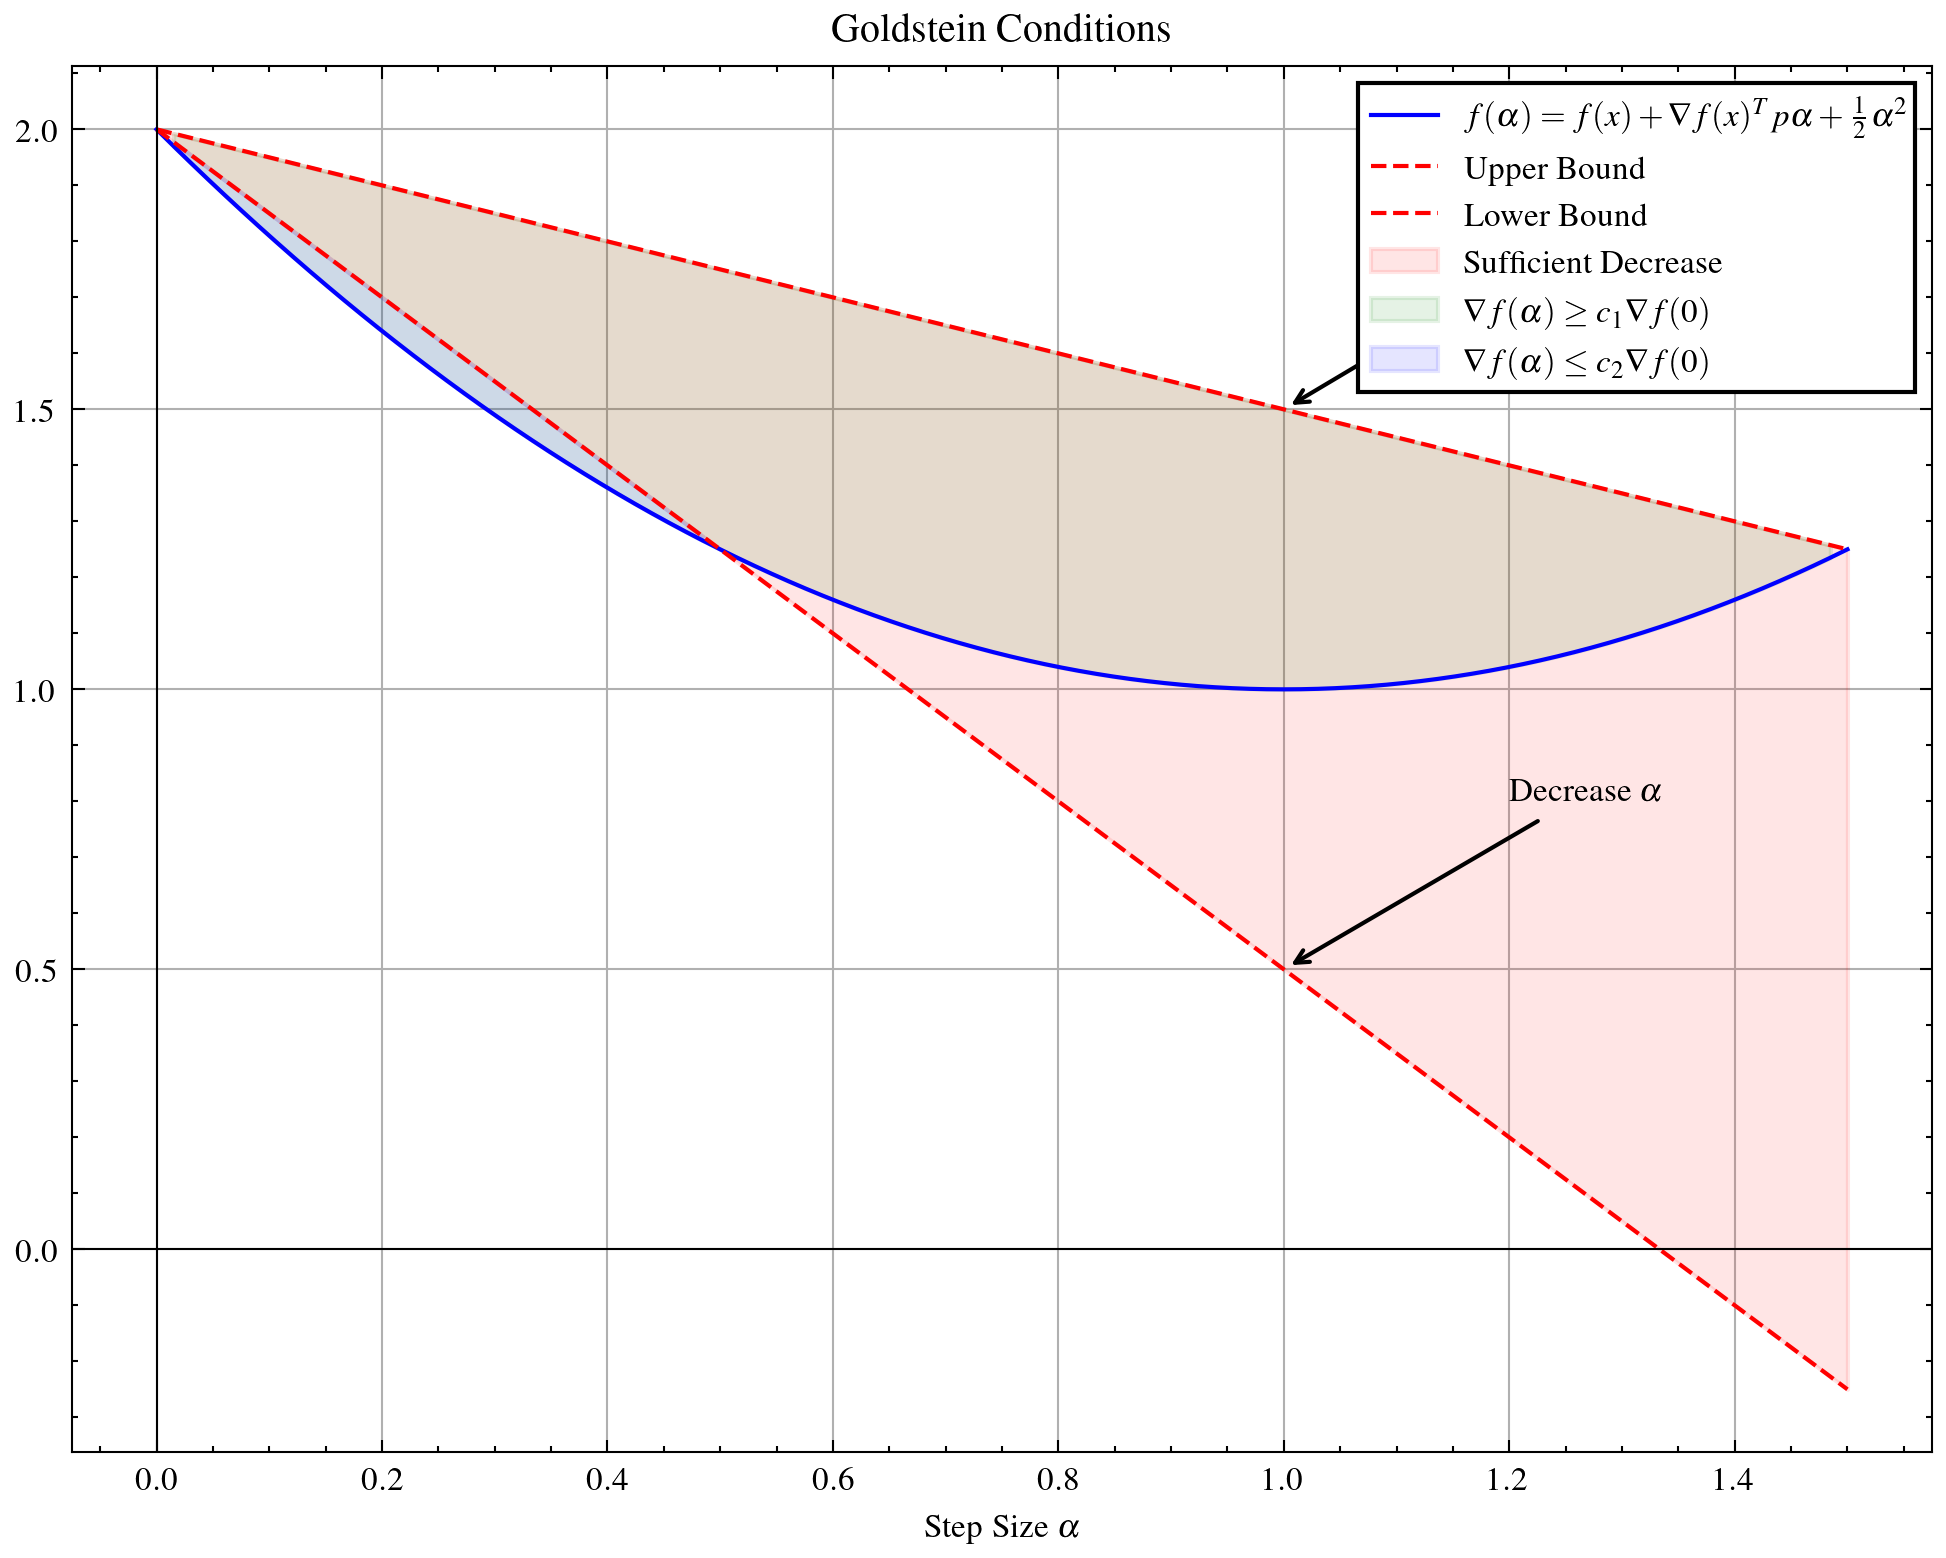
\includegraphics[scale=0.5]{figures/goldstein_conditions.png}
\begin{itemize}
    \item \textbf{Sufficient decrease:} $f(x_k + \alpha p_k) \leq f(x_k) + c_1 \alpha \inner{\nabla f(x_k), p_k}$. If this fails, decrease $\alpha$ because it is too large.
    \item \textbf{Curvature condition:} $f(x_k + \alpha p_k) \geq f(x_k) + c_2 \alpha \inner{\nabla f(x_k), p_k}$. If this fails, increase $\alpha$ because it is too small.
    \item Goldstein conditions are more robust than Armijo conditions.
\end{itemize}

\subsubsection*{Wolfe conditions}
Choose $0 < c_1 < c_2 < 1$.
\begin{itemize}
    \item \textbf{Sufficient decrease:} $f(x_k + \alpha p_k) \leq f(x_k) + c_1 \alpha \inner{\nabla f(x_k), p_k}$. If this fails, decrease $\alpha$ because it is too large.
    \item \textbf{Curvature condition:} $\inner{\nabla f(x_k + \alpha p_k)}{p_k} \geq c_2 \inner{\nabla f(x_k)}{p_k}$. If this fails, increase $\alpha$ because it is too small.
    \item Wolfe conditions are more robust than Goldstein conditions.
\end{itemize}
\subsection{Lecture 6 (24. Januar 2025)}

\section*{Backtracking Linjesøk}
Backtracking Line Search er en metode for å finne en passende skrittlengde \( \alpha \) i iterative optimeringsalgoritmer. Målet er å sikre at skrittet reduserer objektivfunksjonen \( f(\bm{x} + \alpha \bm{p}) \) tilstrekkelig, samtidig som det unngås for små eller ustabile skritt.

\subsection*{Algoritme og Matematisk Formulering}
La \( f: \R^n \to \R \) være kontinuerlig deriverbar, og \( \bm{p} \in \R^n \) en nedstigningsretning (dvs. \( \langle \nabla f(\bm{x}), \bm{p} \rangle < 0 \)). Algoritmen søker \( \alpha > 0 \) som tilfredsstiller \textbf{Armijo-betingelsen}:
\begin{equation}
    f(\bm{x} + \alpha \bm{p}) \leq f(\bm{x}) + c_1 \alpha \langle \nabla f(\bm{x}), \bm{p} \rangle, \quad c_1 \in (0, 1).
\end{equation}

\begin{algorithm}[H]
    \SetAlgoLined
    \DontPrintSemicolon
    \KwIn{$\alpha_0 > 0$, $c_1 \in (0,1)$, $\rho \in (0,1)$}
    \KwOut{$\alpha$}
    $\alpha \leftarrow \alpha_0$\;
    \While{$f(\bm{x} + \alpha \bm{p}) > f(\bm{x}) + c_1 \alpha \langle \nabla f(\bm{x}), \bm{p} \rangle$}{
        $\alpha \leftarrow \rho \alpha$ \tcp*{Reduser skrittlengde}
    }
    \Return{$\alpha$}
    \caption{Backtracking Linjesøk (Armijo)}
\end{algorithm}

\subsection*{Relaterte Betingelser}
\begin{itemize}
    \item \textbf{Armijo-Goldstein}: Legger til en nedre grense for \( \alpha \):
    \begin{equation}
        f(\bm{x}) + c_2 \alpha \langle \nabla f(\bm{x}), \bm{p} \rangle \leq f(\bm{x} + \alpha \bm{p}) \leq f(\bm{x}) + c_1 \alpha \langle \nabla f(\bm{x}), \bm{p} \rangle, \quad 0 < c_1 < c_2 < 1.
    \end{equation}

    \item \textbf{Wolfe-betingelsene}: Inkluderer krumningstilstand:
    \begin{equation}
        \langle \nabla f(\bm{x} + \alpha \bm{p}), \bm{p} \rangle \geq c_2 \langle \nabla f(\bm{x}), \bm{p} \rangle, \quad 0 < c_1 < c_2 < 1.
    \end{equation}
\end{itemize}

\begin{lemma}{Terminering}{}
    Hvis \( f \in C^2 \) er nedre begrenset og \( \bm{p} \) er en nedstigningsretning, terminerer backtracking-algoritmen med en endelig \( \alpha > 0 \).
\end{lemma}

\begin{theorem}{Konvergens for Gradient Descent}{}
    Anta:
    \begin{itemize}
        \item \( f \in C^2 \) med kompakt nivåmengde \( \mathcal{L}_f(\bm{x}_0) = \{\bm{x} \in \R^n \mid f(\bm{x}) \leq f(\bm{x}_0)\} \)
        \item \( \bm{p}_k = -\nabla f(\bm{x}_k) \)
        \item \( \alpha_k \) tilfredsstiller Armijo- eller Wolfe-betingelsene
    \end{itemize}
    Da gjelder:
    \begin{equation}
        \lim_{k \to \infty} \|\nabla f(\bm{x}_k)\| = 0.
    \end{equation}
\end{theorem}

\begin{example}{Kvadratisk Funksjon}{}
    For \( f(\bm{x}) = \frac{1}{2} \bm{x}^\top Q \bm{x} - \bm{b}^\top \bm{x} \) med \( Q \succ 0 \), gir eksakt linjesøk:
    \begin{align*}
        \alpha_k                             & = -\frac{\langle \bm{p}_k, \nabla f(\bm{x}_k) \rangle}{\langle \bm{p}_k, Q \bm{p}_k \rangle}, \\
        \|\bm{x}_{k+1} - \bm{x}^\star\|_Q & \leq \frac{\kappa - 1}{\kappa + 1} \|\bm{x}_k - \bm{x}^\star\|_Q,
    \end{align*}
    hvor \( \kappa = \operatorname{cond}(Q) = \frac{\lambda_{\max}(Q)}{\lambda_{\min}(Q)} \).
\end{example}

\begin{example}{Rosenbrock-funksjonen: Hessian}{}
    For \( f(x,y) = (1 - x)^2 + 100(y - x^2)^2 \) har Hessianen i minimum \( \bm{x}^\star = (1,1) \) formen:
    \begin{equation}
        H_f(1,1) = \begin{bmatrix} 802 & -400 \\ -400 & 200 \end{bmatrix}.
    \end{equation}
    Kondisjonstallet \( \kappa \approx 2500 \) forklarer treg konvergens for gradientdescent.
\end{example}


\subsection{Lecture 7 (27. Januar 2025)}

\paragraph{Goal for today}
\begin{itemize}
    \item Newton's Method:
    \begin{itemize}
        \item Definition and convergence rate
        \item Combination with line search
        \item Necessary modifications
    \end{itemize}
\end{itemize}

\section*{Newton's Method}

\paragraph{Background}
Assume \(G: \R^d \to \R^d\). We want to solve \(G(x) = 0\).

Newton's method is an iterative procedure for finding the roots of a differentiable function \(G: \R^d \to \R^d\). 
It uses the first-order Taylor (linear) approximation of \(G\) at the current point \(x_k\).

\begin{definition}{Newton's Method}{}
    The iteration is defined by
    \begin{align*}
        x_{k+1} &= x_k - \bigl(D G(x_k)\bigr)^{-1} G(x_k),
    \end{align*}
    where \(D G(x_k)\) is the derivative (Jacobian) of \(G\) at \(x_k\). If \(G\) is the gradient of a scalar function \(f\), then \(DG(x_k) = H_f(x_k)\), the Hessian of \(f\).
\end{definition}

\paragraph{Convergence Theory}
If \(G\in \mathcal{C}^2\), then this iteration converges locally \emph{quadratically} to 
a solution \(x^\star\) of \(G(x) = 0\), provided that \(D G(x^\star)\) is invertible.

\begin{remark}
    Quadratic convergence means there exist constants \(C>0\) and \(\delta>0\) such that for all \(k\) with \(\|x_k - x^\star\|\le \delta\),
    \[
        \|x_{k+1} - x^\star\| \;\le\; C \,\|x_k - x^\star\|^2.
    \]
\end{remark}

\subsection*{Application to Optimization}

We apply Newton's method to solve \(\nabla f(x) = 0\). That is, to find stationary points of a function \(f:\R^d \to \R\).

\paragraph{Basic Method}
\begin{itemize}
    \item Newton iteration:
    \[
      x_{k+1} \;=\; x_k \;-\; H_f(x_k)^{-1} \,\nabla f(x_k).
    \]
    \item Alternatively, set up the system \(H_f(x_k)\,p_k = -\,\nabla f(x_k)\) and then \(x_{k+1} = x_k + p_k\).
    \item Convergence: If \(f\in \mathcal{C}^3\) and \(H_f(x^\star)\) is nonsingular at the local minimizer \(x^\star\), the method converges locally quadratically.
\end{itemize}

\begin{algorithm}[H]
\caption{Basic Newton's Method}
\label{alg:newton-basic}
\KwInput{Starting point $x_0$, tolerance $\epsilon > 0$}
\KwOutput{Approximate solution $x_k$}
$k \gets 0$\;
\While{$\|\nabla f(x_k)\| > \epsilon$}{
    Compute Hessian $H_f(x_k)$\;
    Solve $H_f(x_k)\,p_k = -\,\nabla f(x_k)$\;
    $x_{k+1} \gets x_k + p_k$\;
    $k \gets k + 1$\;
}
\KwRet{$x_k$}\;
\end{algorithm}

\paragraph{Global Convergence Strategy}
\begin{enumerate}
    \item Combine with a line search.
    \item Define \(p_k\) by solving \(H_f(x_k)\,p_k = -\nabla f(x_k)\).
    \item Choose a step length \(\alpha_k > 0\).
    \item Update \(x_{k+1} = x_k + \alpha_k \, p_k\).
\end{enumerate}

\begin{algorithm}[H]
\caption{Globally Convergent Newton's Method}
\label{alg:newton-global}
\KwInput{Starting point $x_0$, tolerances $\epsilon, c > 0$, reduction factor $\rho \in (0,1)$}
\KwOutput{Approximate solution $x_k$}
$k \gets 0$\;
\While{$\|\nabla f(x_k)\| > \epsilon$}{
    Compute Hessian $H_f(x_k)$\;
    Solve $H_f(x_k)\,p_k = -\nabla f(x_k)$\;
    $\alpha_k \gets 1$\;
    \While{$f(x_k + \alpha_k p_k) > f(x_k) + c\,\alpha_k\,\nabla f(x_k)^\top p_k$}{
        $\alpha_k \gets \rho\,\alpha_k$\;
    }
    $x_{k+1} \gets x_k + \alpha_k p_k$\;
    $k \gets k + 1$\;
}
\KwRet{$x_k$}\;
\end{algorithm}

\paragraph{Descent Direction Condition}
If \(H_f(x_k)\) is positive definite, then
\[
    \langle p_k, \nabla f(x_k)\rangle
    \;=\;
    -\,\langle H_f(x_k)^{-1}\,\nabla f(x_k),\,\nabla f(x_k)\rangle
    \;<\; 0,
\]
so \(p_k\) is a descent direction for the line search.

\paragraph{Modified Newton's Method}
If \(H_f(x_k)\) is not positive definite, or if \(\langle \nabla f(x_k), p_k\rangle \geq 0\), then the line search may fail. One approach is to modify the Hessian or switch to a different direction:

\begin{itemize}
    \item First compute \(p_k = -\,H_f(x_k)^{-1}\,\nabla f(x_k)\).
    \item If \(\langle \nabla f(x_k),\,p_k\rangle \;\ge\; \varepsilon \,\|\nabla f(x_k)\|\,\|p_k\|\) for some \(\varepsilon > 0\), switch to \(p_k = -\,\nabla f(x_k)\).
    \item Alternatively, modify the Hessian so it is sufficiently positive definite (e.g.\ shift its eigenvalues).
\end{itemize}

\begin{algorithm}[H]
\caption{Modified Newton's Method with Hessian Modification}
\label{alg:newton-modified}
\KwInput{Starting point $x_0$, tolerances $\epsilon, \varepsilon > 0$}
\KwOutput{Approximate solution $x_k$}
$k \gets 0$\;
\While{$\|\nabla f(x_k)\| > \epsilon$}{
    Compute Hessian $H_f(x_k)$\;
    Compute eigendecomposition $H_f(x_k) = U\,\Lambda\,U^\top$\;
    $M \gets \text{diag}\bigl(\max\{\lambda_1, \varepsilon\}, \ldots, \max\{\lambda_d, \varepsilon\}\bigr)$\;
    $p_k \gets -\,U\,M^{-1}\,U^\top\,\nabla f(x_k)$\;
    \uIf{$\nabla f(x_k)^\top p_k < -\,\varepsilon\,\|\nabla f(x_k)\|\|p_k\|$}{
        Use $p_k$ as the search direction\;
    }
    \Else{
        $p_k \gets -\,\nabla f(x_k)$\;
    }
    % In a global method, we would then do a line search on p_k:
    %   x_{k+1} = x_k + alpha_k p_k
    % but here it is omitted for brevity.
    $x_{k+1} \gets x_k + p_k$\;
    $k \gets k + 1$\;
}
\KwRet{$x_k$}\;
\end{algorithm}

\paragraph{Alternative Interpretation of Newton's Method}
Newton's method can also be viewed via a second-order Taylor expansion of \(f\) around \(x_k\):

\begin{enumerate}
    \item Approximate \(f\) by 
    \[
        m_k(p) \;=\; f(x_k) \;+\; \langle \nabla f(x_k),\, p\rangle \;+\; \tfrac12\,\langle H_f(x_k)\,p,\,p\rangle.
    \]
    \item Find \(p_k\) by minimizing \(m_k(p)\). 
    \[
      \nabla m_k(p_k) \;=\; \nabla f(x_k) \;+\; H_f(x_k)\,p_k \;=\; 0
      \quad\Longrightarrow\quad
      p_k = -\,H_f(x_k)^{-1}\,\nabla f(x_k).
    \]
    \item If \(H_f(x_k)\) is not positive definite, one modifies it to be positive definite (e.g.\ shifting eigenvalues).
\end{enumerate}

The \emph{modified Newton's method} then reads \(x_{k+1} = x_k + \alpha_k\,p_k\) with \(\alpha_k>0\) found by a line search and \(p_k\) given by one of the strategies above.

\paragraph{Quadratic Convergence Criterion}
Quadratic convergence holds precisely when, near \(x^\star\), we use
\[
    p_k \;=\; -\,H_f(x_k)^{-1}\,\nabla f(x_k)
    \quad\text{and}\quad
    \alpha_k \;=\; 1.
\]
In particular, for \(\alpha_k = 1\) to be acceptable in the line search once \(x_k\) is close to \(x^\star\), the Hessian near \(x^\star\) must be uniformly positive definite (so all eigenvalues \(\ge \varepsilon > 0\)), and the line search parameters (e.g.\ the Armijo or Wolfe constants) must allow a full step.

\section*{Conjugate Gradient Methods}

We now focus on the special case of minimizing the quadratic function
\[
\Phi(x) \;:=\; \tfrac12\,\langle x,\;Q\,x\rangle \;-\; \langle b,\;x\rangle,
\]
where \(Q \in \R^{d\times d}\) is symmetric positive definite and \(b \in \R^d\). In exact arithmetic, the \emph{Conjugate Gradient} (CG) method can solve this problem in at most \(d\) steps.

With exact line search, the update is
\[
x_{k+1} 
\;=\; x_k \;-\; \frac{\langle Q\,x_k - b,\;p_k\rangle}{\langle Q\,p_k,\;p_k\rangle}\,p_k,
\]
which ensures 
\[
\langle \nabla \Phi(x_{k+1}),\;p_k\rangle \;=\; 0.
\]
In particular, for a gradient method we would have \(\nabla \Phi(x_{k+1}) \propto p_{k+1}\). Orthogonality conditions arise naturally here.

\paragraph{Conjugate Directions}
A set of vectors \(\{p_0, p_1, \dots, p_{d-1}\}\subset \R^d\) is \emph{conjugate} with respect to \(Q\) if
\[
    \langle p_i,\;Q\,p_j\rangle \;=\; 0 \quad\text{for}\quad i\neq j.
\]
Equivalently, the vectors are mutually orthogonal under the inner product \(\langle u, v \rangle_Q := \langle u, Q\,v\rangle\).

\begin{lemma}{Conjugate Directions}{}
    Let \(\{p_0,\ldots,p_{d-1}\}\) be a conjugate basis of \(\R^d\). Consider the iteration
    \[
    x_{k+1} \;=\; x_k + \alpha_k\,p_k
    \quad\text{with}\quad
    \alpha_k \;=\; -\,\frac{\langle r_k,\;p_k\rangle}{\langle Q\,p_k,\;p_k\rangle},
    \]
    where \(r_k = Q\,x_k - b\). Then \(x_d = x^\star = Q^{-1}b\). In other words, the exact solution is reached in at most \(d\) steps.
\end{lemma}

\begin{proof}{}{}
Since \(\{p_0,\ldots,p_{d-1}\}\) is a basis, there exist scalars \(\sigma_k\) such that
\[
x^\star - x_0 
\;=\; \sum_{k=0}^{d-1} \sigma_k\,p_k.
\]
Also,
\[
x_d - x_0 
\;=\; \sum_{k=0}^{d-1} \alpha_k\,p_k.
\]
To show \(x_d = x^\star\), it suffices to prove \(\sigma_k = \alpha_k\) for all \(k\). Indeed,
\[
    \sigma_l 
    \;=\; \frac{\langle x^\star - x_0,\;Q\,p_l\rangle}{\langle p_l,\;Q\,p_l\rangle}
    \;=\; \frac{\langle Q\,(x^\star - x_0),\;p_l\rangle}{\langle p_l,\;Q\,p_l\rangle}
    \;=\; \frac{\langle b - Q\,x_0,\;p_l\rangle}{\langle p_l,\;Q\,p_l\rangle}.
\]
Also,
\[
    \alpha_l
    \;=\; -\,\frac{\langle r_0,\;p_l\rangle}{\langle Q\,p_l,\;p_l\rangle},
    \quad\text{where}\quad r_0 \;=\; Q\,x_0 - b.
\]
Careful manipulation (and using the fact that \(\langle p_i, Q\,p_j\rangle=0\) for \(i\neq j\)) shows \(\sigma_l = \alpha_l\). Hence \(x^\star = x_d\).
\end{proof}

\paragraph{The CG Iteration}
The Conjugate Gradient method constructs a sequence of conjugate directions by choosing
\[
p_0 = -\,r_0 \;=\; b - Q\,x_0,
\quad
p_{k+1} = -\,r_{k+1} + \beta_k\,p_k
\]
with \(\beta_k\) chosen so that \(\langle p_{k+1},\,Q\,p_k\rangle=0\). One can show this leads to convergence in at most \(d\) steps for solving \(Q\,x = b\) in exact arithmetic.

\subsection{Lecture 8 (31. February 2025)}

\textbf{Goals:}
\begin{enumerate}
    \item \textbf{CG Convergence:} Theoretical guarantees and convergence speed
    \item \textbf{Efficient Reformulation:} Practical CG improvements
    \item \textbf{Nonlinear Extension:} Fletcher--Reeves method
    \item \textbf{Step Length Selection:} Optimal step size strategies
    \item \textbf{Alternative Methods:} Polak--Ribière and Hestenes--Stiefel variants
\end{enumerate}

\begin{theorem}{}{}
    As long as \(r_k \neq 0\), we have that:
    \begin{itemize}
        \item \(\inner{r_k, r_e}=0 \forall l = 0,...,k-1 \)
        \item \(\spann\{p_0,\ldots, p_k\} = \spann\{r_0, \ldots, r_k\} = \spann\{r_0, Qr_0, Q^2r_0,\ldots, Q^k r_0\}\)
        \item \(\inner\{p_k, Qp_l\} = 0 \forall \; l=0,\ldots,k-1\)
        \item In particular 
    \end{itemize}
\end{theorem}

\begin{lemma}{}{}
    Assume that \alpha satisfies in each step the strong curvature condition:
    \[
    \left|\inner{}\right|
    \]

\end{lemma}

\subsubsection{Forelesning 9 (3. Februar 2025)}

\begin{definition}{Newton's Method}{newton-method}
    \[
    x_{k+1} = x_k - [\nabla^2 f(x_k)]^{-1} \nabla f(x_k) = x_k - H_k^{-1} \nabla f(x_k) = x_k + p_k
    \]
    where \( H_k \) is the Hessian matrix.
\end{definition}

But computing the Hessian matrix is expensive, so we use the \textbf{quasi-Newton} method instead.

\section*{Quasi-Newton Methods}
The quasi-Newton method is an iterative optimization algorithm that approximates the Hessian matrix using rank-one updates. 
This approach avoids the computational cost of computing the exact Hessian matrix and can provide faster convergence rates.
\begin{definition}{Quasi-Newton Method}{quasi-newton}
    \[
    x_{k+1} = x_k - B_k^{-1} \nabla f(x_k) = x_k + p_k
    \]
    where \( B_k \) is an approximation of the Hessian matrix.
\end{definition}

\begin{algorithm}[H]
    \caption{Quasi-Newton Method}
    \label{alg:quasi-newton}
    \SetKwFunction{QuasiNewton}{QuasiNewton}
    \QuasiNewton{$x_0$, $B_0$, $f$, $\nabla f$, $\epsilon$}\;
    \While{$\norm{\nabla f(x_k)} > \epsilon$}{
        Compute the search direction $p_k = -B_k^{-1} \nabla f(x_k)$\;
        Choose the step size $\alpha_k$ by line search\;
        Update the current point $x_{k+1} = x_k + \alpha_k p_k$\;
        Update the approximation $B_{k+1}$ of the Hessian matrix\;
    }
    \KwRet{$x_k$}\;
\end{algorithm}

\paragraph{Update Formulas}

\begin{itemize}
    \item \textbf{DFP update}: \( B_{k+1} = B_k + \frac{y_k y_k^T}{y_k^T s_k} - \frac{B_k s_k s_k^T B_k}{s_k^T B_k s_k} \)
    \item \textbf{BFGS update}: \( B_{k+1} = B_k + \frac{(y_k y_k^T)}{y_k^T s_k} - \frac{(B_k s_k)(B_k s_k)^T}{s_k^T B_k s_k} \)
    \item \textbf{SR1 update}: \( B_{k+1} = B_k + \frac{(y_k - B_k s_k)(y_k - B_k s_k)^T}{(y_k - B_k s_k)^T s_k} \)
    \item \textbf{Broyden update}: \( B_{k+1} = B_k + \frac{(y_k - B_k s_k - B_k^T y_k)(s_k^T B_k)}{s_k^T B_k s_k} \)
\end{itemize}

\subsection*{SR1 Update}
The SR1 update is a rank-one update that approximates the Hessian matrix using the following formula:
\[
B_{k+1} = B_k + \frac{(y_k - B_k s_k)(y_k - B_k s_k)^T}{(y_k - B_k s_k)^T s_k}
\]
where \( s_k = x_{k+1} - x_k \) and \( y_k = \nabla f(x_{k+1}) - \nabla f(x_k) \).







\end{document}
